\documentclass[11pt, a4paper, twoside]{book}

\setlength{\topmargin}{2pt} \setlength{\headheight}{15pt}
\setlength{\headsep}{25pt} \setlength{\textheight}{640pt}
\setlength{\footskip}{25pt}
\setlength{\hoffset}{0pt}
\setlength{\oddsidemargin}{0pt} \setlength{\oddsidemargin}{3pt}
\setlength{\evensidemargin}{0pt} \setlength{\evensidemargin}{30pt}
\setlength{\textwidth}{430pt}
\setlength{\marginparsep}{0pt} \setlength{\marginparwidth}{0pt}
\usepackage[french]{babel}
\usepackage[utf8]{inputenc}
%\usepackage[IT]{fontenc}
\usepackage{graphicx}
\graphicspath{ {images/} }
\usepackage[margin=1.25in]{geometry}

\usepackage{longtable}
\usepackage{float}
\usepackage{textcomp}
\usepackage{amsmath}
\usepackage{pdfpages}

%start of title
{\title{
%include the logo
\begin{figure}[h]
\centering			

\includegraphics[width=0.5\textwidth]{logo}
\end{figure}
ÉCOLE NATIONALE DES SCIENCES APPLIQUÉES DE KÉNITRA \\  \vspace*{1truecm} Moroccan foundation for Advanced Science, Innovation and Research \\ 
(MAScIR) \\
\vspace*{1truecm} Rapport de Projet de Fin d'Année \\ \vspace*{0.5truecm} \textbf{Étude et réalisation d'un system RFID}} 
%end of title

\author{Réalisé par : \\ Otmane BOUAYAD \vspace*{1truecm} \\ Encadré par : \\ Mme Ilham BOUZIDA : Encadrante professionnelle\\ }
\date{(Du 15 Février au 25 Août  2016)}

\begin{document}
\maketitle
\pagestyle{plain}
%Dedicas

\chapter*{Dédicace}

I would like to dedicate this work to my wife, Oumaima, for her love, encouragement, and continuous support,my parents, who has taught me many things in life and include the one thing I’ve tried to live by: 
\emph{“Never give up on your dreams. Hard work and diligence will see you through so long as you never give up.”}
 So it is with all my love, respect, and admiration that I dedicate this to you.My sister and my best friends forever Reda and Nouhaila,my future engineers. remember
\emph{“Accomplishment is product of thoughts, mind is everything”.}

%remerciment
\chapter*{Remerciements}
\addcontentsline{toc}{section}{Remerciements}
\emph{
Avant tout développement sur cette expérience professionnelle, il apparaît opportun 
de commencer ce rapport de stage par des remerciements, à ceux qui nous ont beaucoup 
aidé au cours de ce stage, et même à ceux qui ont eu la gentillesse de faire de ce stage un 
moment très profitable.\\\\}
\emph{
Aussi, Nous tenons plus particulièrement à remercier Mme Ilham
BOUZIDA, ingénieur qualité dans l’équipe packaging à MAScIR, et à M. Brahim LAKSSIR, chef de service packaging à MAScIR,nos maîtres de stage qui ont la part de lion dans notre formation et accompagnement professionnels avec beaucoup de patience et de savoir-faire.\\\\ }
\emph{Je souhaite remercier mon promoteur et mon encadrant à l'école Pr. Tomader MAZRI pour ses instructions et son aide lors du stage.\\\\}
\emph{
Finalement , nous remercions l’ensemble des employés de la Fondation MAScIR pour les conseils qu’ils ont pu nous prodiguer au cours de ce stage.
}\\\\
\emph{Enfin, j’adresse tous mes remerciements les plus sincères à tous les enseignants de l’ENSA de Kenitra pour avoir contribué à la formation que j’ai acquise lors de mon cursus.}
%include the table of content please
\tableofcontents

%include the liste of figure please
\listoffigures

\listoftables

\chapter*{Introduction}
\addcontentsline{toc}{section}{Introduction}
Le terme RFID englobe toutes les techniques qui utilisent les ondes radio pour identifier automatiquement des objets ou des personnes.
Le système RFID autrement dit l'identification par radio fréquence est une technique qui permet de mémoriser et de récupérer des informations à distance grâce à une étiquette qui émet des ondes radio.\\
Le système RFID (audiofréquence identification) est une technique très attractive pour l'entreprise qui offre la possibilité d'une gestion automatique du nombre conséquent d'informations qu'elle doit traiter. Les équipements adaptés à ce système permettent de synchroniser les flux physiques avec les flux d'informations.\\\\
Dans le cadre du projet de fin d'études, j'ai eu l'opportunité de travailler sur cette technique avec la fondation MAScIR qui occupe une position leader sur le marché de la micro-électronique.\\\\
Le projet de fin d’études porte alors, sur l'étude et la réalisation d’une solution RFID UHF qui assure l’identification et la traçabilité des entrées et sorties des palettes. Choisire les tags adaptés aux besoins en respectant les conditions d’utilisation et type de lecteur. Devolopper un logiciel de gestion des palettes. D’autre part, la réalisation d’un transpondeur RFID UHF et une application Android pour gestion du secteur d'agriculture.\\\\
Le mémoire que je présente est organisé en 6 chapitres.

\begin{itemize}
\item Chapitre 1: présentation de l'entreprise d'accueil ainsi qu'une description du déroulement du stage.
\item Chapitre 2: contexte général du Projet.
\item Chapitre 3: étude bibliographique, et principe de fonctionnement d’un système RFID. 
\item CHapitre 4: conception et test de la partie logitiel.
\item Chapitre 5: etude du besoin du secteur agriculture et developement de l'application Android.
\item Chapitre 6: conception d'un transpondeur RFID UHF.
\end{itemize}

\pagestyle{plain}

\chapter{Persentation de l'entreprise d'accueil}
\pagestyle{headings}
\section{Présentation générale de MAScIR}
MAScIR (Moroccan foundation for Advanced Science, Innovation and Research) est un organisme de recherche à caractère scientifique et technologique. Il est voué à la recherche en nanotechnologie, en biotechnologie, en technologie numérique, en microélectronique, en énergie et en environnement, la fondation se veut présenter là où les enjeux de la société l’exigent.\\

La figure suivante montre l’emplacement de l’entreprise.

\begin{figure}[h]
\centering
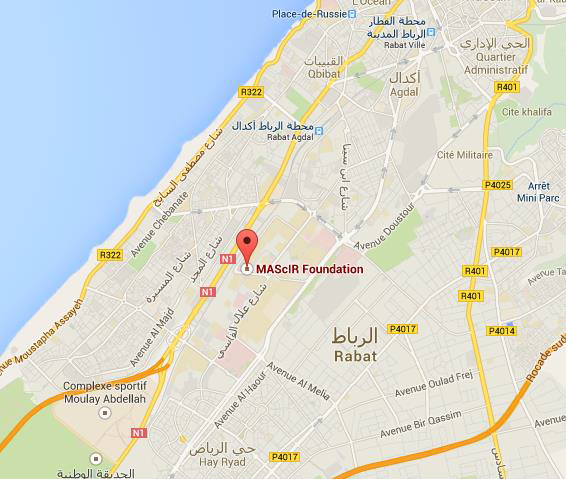
\includegraphics[width=0.75\textwidth]{mascir_map}
\caption{Localisation de la fondation MAScIR}
\end{figure}

Rassemblant d’éminents chercheurs des quatre coins du monde, MAScIR regroupe des équipes scientifiques œuvrant dans des domaines innovants et complémentaires et met à leur disposition une infrastructure scientifique de pointe.\\

Initialement fondée en 2007 par le Gouvernement Marocain en tant que fondation à but non lucratif MAScIR a continué son expansion en créant :

\begin{description}
\item[MAScIR MicroElectronics] a pour objectif de devenir un centre de Recherche et Développement dans le domaine de la microélectronique.
\item[MAScIR BioTechnology] deuxième centre inscrit dans MAScIR œuvrant dans le domaine de la biotechnologie : recherche et développement des médicaments ou des biocides.
\item[NanoTechnology] qui a pour mission de mener des recherches appliquées, innovantes et à la fine pointe de la technologie dans le domaine des nanomatériaux et des nanotechnologies. Ces recherches sont menées par une équipe internationale de haut calibre travaillant dans un environnement unique et utilisant une infrastructure de pointe.
\end{description}

\subsection{Partenaires de la foundation}
Les principaux partenaires de la fondation MASCIR MicroElectronics sont :
\begin{description}
\item[Lear Corporation] est l’un des principaux fournisseurs mondiaux de sièges automobiles et les systèmes de gestion de l’énergie électrique.
\item[Thales] figure parmi les leaders européens de la fabrication et de la commercialisation d'équipements et de systèmes électroniques destinés aux secteurs de l'aérospatial, du transport, de la défense et de la sécurité.
\item[OCP] est un acteur incontournable sur le marché des phosphates et de ses produits dérivés. Présent sur toute la chaine de valeur, il est le premier exportateur de cette matière dans le monde.
\item[COSUMAR] est un groupe marocain, filiale de la Société nationale d'investissement, spécialisé dans l'extraction, le raffinage et le conditionnement du sucre sous différentes formes. Il est devenu l'unique opérateur sucrier marocain après l'acquisition de SUTA, SUCRAFOR, SUNABEL et SURAC en 2005.
\item[STERIMED] est une société spécialisée dans le domaine de l’eau et des technologies de l’environnement. Son objectif est d’accompagner les entreprises et collectivités dans la résolution des problématiques liées à l’eau, l’environnement.
\end{description}

\subsection{Structure et hiérarchie}
La Fondation est gérée par un conseil d’administration qui est investi de pouvoirs de gestion à cet égard. Le Conseil dispose de quatre comités distincts : un Comité d’Investissement, un Comité de suivi, un comité de vérification et un Comité de Rémunération; qui assurent une gestion rapprochée des sujets relatifs à leur mission.
\begin{description}
\item[Conseil d'administration] détermine les orientations stratégiques de MAScIR et veille à leur mise en œuvre dans des réunions régulières. En prenant des décisions, le Conseil compte sur le travail des comités spécialisés.
\item[Comité de vérification] le rôle principal du Comité d'audit est de permettre à la Commission de veiller à la qualité des contrôles internes et l'intégrité de l'information divulguée aux intervenants et aux partenaires.
\item[Comité des Rémunérations] est responsable de faire des recommandations au Conseil sur la nomination des administrateurs. Il est également responsable de l'examen de la politique en matière de rémunération de la haute direction au sein de MAScIR.
\item[Comité de suivi] surveille la mise en œuvre effective et correcte des projets dans le cadre de l'accord signé entre MAScIR et le Gouvernement marocain.
\item[Comité d'Investissement] assiste le Conseil d'administration dans l'accomplissement de sa responsabilité de surveillance pour les actifs d'investissement liés à l'équipement scientifique.
\end{description}

\section{Présentation du département microélectronique}
MAScIR Micro est un centre d’innovation et développement de technologie dans le domaine de la microélectronique. Il se focalise sur la simulation, les tests, le design, le packaging, la qualification et le prototypage des produits microélectroniques.
\subsection{Mission}
Le programme Microélectronique a réuni une équipe de direction de classe mondiale pour assurer la traction initiale sous licence des technologies de pointe qui sont disponibles pour une utilisation immédiate. \\

Le programme Microélectronique a réuni une équipe de direction de classe mondiale pour assurer la traction initiale sous licence des technologies de pointe qui sont disponibles pour une utilisation immédiate. \\

MAScIR Micro fournit des services pour des clients industriels, mais elle développe aussi son propre business dans les domaines suivants :
\begin{itemize}
\item L’intégration et la miniaturisation des systèmes microélectroniques.
\item L’analyse de fiabilité et défaillance des produits.
\item Modélisation des systèmes complexes.
\item Prototypage et industrialisation des produits innovants.
\item Industrialisation des idées et résultats académiques.
\end{itemize}

\subsection{Laboratoires}
Le département microélectronique de MAScIR possède plusieurs laboratoires équipés de technologie avancée :
\begin{itemize}
\item Salle blanche
\item Laboratoire de fiabilité et analyse de défauts
\item Laboratoire électronique
\end{itemize}

\begin{figure}[h!]
\centering
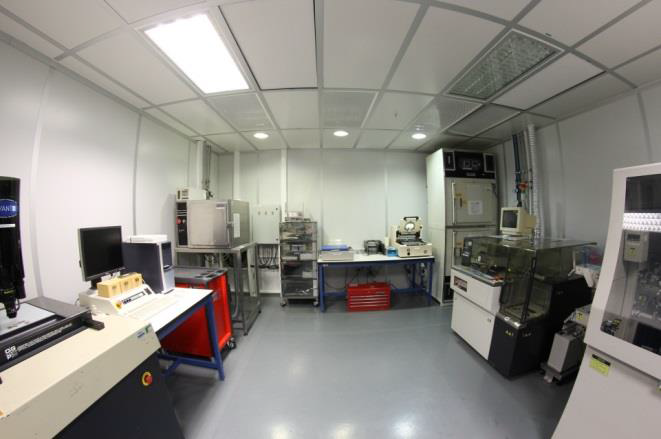
\includegraphics[width=0.75\textwidth]{cleanroom}
\caption{Salle blanche}
\end{figure}

\begin{figure}[h!]
\centering
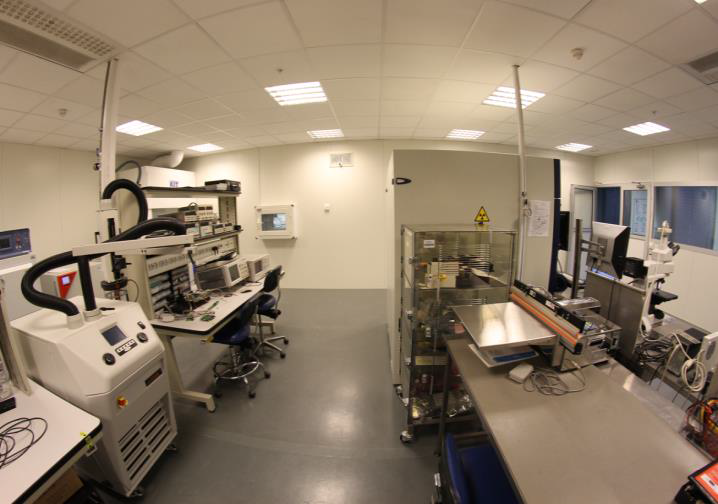
\includegraphics[width=0.75\textwidth]{labo}
\caption{Laboratoire de fiabilité et analyse de défauts}
\end{figure}

\subsection{Équipements}
\begin{itemize}
\item Ligne CSP (Chip Scaled Packaging)
\item Ligne SMT (Surface Mount Technology)
\item SAM (Scanning Accoustic Microscope)
\item X-Ray
\item Chambres climatiques
\end{itemize}

Pour plus d'informations, visiter le site de l'entreprise : \texttt{http://www.mascir.ma}.

\section{Description et déroulement du stage}
\subsection{Activités exercées}
Durant ce stage de fin d’études, j’ai eu l’opportunité de côtoyer le monde industriel et plus précisément de la microélectronique ce qui m’a permis d’assister et participer à plusieurs missions et projets que ce soit au sein de MAScIR ou à l’extérieur.\\

Mis à part le travail sur mon projet, j’ai pu suivre le processus du packaging allant du découpage wafer au marquage boitier et sciage.\\

Parallèlement, J’ai assisté à des manœuvres de vérification de qualité des produits livrés à MAScIR.\\

Par ailleurs, j’ai pu bénéficier d’un encadrement étroit en préparant des réunions pour garantir un bon état d’avancement du projet.

\subsection{Répartition des tâches}
%you need to revise mistakes
\noindent
\textsc{1\textsuperscript{ère} et 2\textsuperscript{ème} semaines :}
\begin{itemize}
\item Visite du local et réunions pour cerner le projet.
\item Bibliographie sur les system RFID.
\end{itemize}
\textsc{3\textsuperscript{ème} et 4\textsuperscript{ème} semaines :}
\begin{itemize}
\item Etude du marcher et choix des tags et lecteur rfid.
\item Participer à la résolution des problèmes du lecteur existant.
\end{itemize}
\textsc{5\textsuperscript{ème} et 6\textsuperscript{ème} semaine :}
\begin{itemize}
\item Etude et familiarisation avec le language \emph{.NET C\#}
\item Realisation d'un prototype de test de lecture de tages.
\end{itemize}
\textsc{7\textsuperscript{ème} et 8\textsuperscript{ème} semaine :}
\begin{itemize}
\item Proposition d'algorithme d'amelioration des performance de la commincation client-lecteur
\item Implementation final du prototype du nouveau protocol de communiation client lecteur.
\end{itemize}
\textsc{9\textsuperscript{ème} semaine :}
\begin{itemize}
\item Developpement d'une interface utilisateur pour le control du flux des donnee et gestion de stockage.
\item Etude du marcher marcaine de l'agrigulture et Etude de besoin .
\end{itemize}
\textsc{10\textsuperscript{ème} et 11\textsuperscript{ème} semaine :}
\begin{itemize}
\item Developpement de la Version une de l'application SmartFlah.
\item Amelioration de la version une de l'application SmartFlah
\end{itemize}
\textsc{12\textsuperscript{ème} et 13\textsuperscript{ème} semaine :}
\begin{itemize}
\item Etude Profondis sur les Tag RFID UHF.
\item Realisation du 1er prototype d'antenne UHF RFID
\end{itemize}
\textsc{14\textsuperscript{ème} et 15\textsuperscript{ème} semaine :}
\begin{itemize}
\item Etude des methode d'optimisation du tailet performance d'antenne.
\item simulation sur CST du 2eme prototype d'antenne
\end{itemize}
\textsc{16\textsuperscript{ème} et 17\textsuperscript{ème} semaine :}
\begin{itemize}
\item simulation sur CST du 3eme prototype d'antenne
\item Redaction du rapport
\end{itemize}



\chapter{Contexte Général du projet}
Le but de ce chapitre est de présenter la problématique du projet, le cahier des charges, la démarche suivie pour répondre au besoin de l’ensemble des parties prenantes du projet et le plan d’action.
\section{Cahier des charges}
\subsection{Objectif}
L’objectif de ce projet est l'étude et la réalisation d’une solution RFID UHF qui assure l’identification et la traçabilité des entrées et sorties des palettes. Choisire les tags adaptés aux besoins en respectant les conditions d’utilisation et type de lecteur et de devolopper un logiciel de gestion des palettes. 
Et comme deuxième axe,la réalisation d’un transpondeur RFID UHF et une application Android pour gestion du secteur d'agriculture qui permet a
l’utilisateur de profiter des fonctions offerte par le système à distance. \\
\subsection{Cachier des charges}
Assurer l’identification et la traçabilité des entrées / sorties palettes
\begin{itemize}
\item Choix des puces/tags adaptés aux besoins (conditions d’utilisation et type de lecteur).
\item Etablir un pgr de gestion des palettes en assurant la traçabilité de leur mouvement.
\item Réalisation et test d’un proto.\\
\end{itemize}
\subsection{Mise au point de la problématique}
Ce projet consiste à développer un système de traçabilité des entrées et sorties des palettes. Trouver les causes racines, choisir les solutions optimales pour un problème ou une situation nécessite une grande compréhension du problème. Dans ce sens, la méthode QQOQCP permet d'avoir des informations élémentaires suffisantes sur toutes les dimensions du problème, pour identifier ses aspects essentiels.\\\\\\\
        
\begin{longtable}{|l|c|}
  \hline
  Quoi & Activité : Développement d’un un système de traçabilité \\
       &  Produit : logiciel de reconnaissance faciale, Application Android, Tag UHF \\
  \hline
  Qui & Division : Client MAcIR\\
  \hline
  Où & MAcIR\\
  \hline
  Quand & Du 15/02/2016 au 15/06/2015\\
  \hline
  Comment & Etat d’art sur les techniques RFID \\
          &  existantes afin de développer un autre plus adapté.\\
  \hline
  Pourquoi & Fournir un système de traçabilité des entrées et sorties des palettes.\\
  \hline
  
\caption{QQOQCP}
\end{longtable}

\section{Deroulement chronologique du stage}
Durant les 4 mois de mon stage, les tˆaches relatives `a mon projet de stage sont organis de la facon suiavante:
\subsection{Etapes	de	réalisaion}
\begin{longtable}{|p{0.35\textwidth}|p{0.2\textwidth}|p{0.2\textwidth}| p{0.15\textwidth}|}
\hline
\textbf{Tâche} & \textbf{Date de début} & \textbf{Date de fin} & \textbf{Durée} \\
\hline
Visites et réunions & 16/02/16 & 18/02/16 & 3 jours \\
\hline
Bibliographie RFID & 15/02/16 & 26/02/16 & 10 jours \\
\hline
Etude du marcher et choix des tags et lecteur rfid & 29/02/16 & 04/03/16 & 5 jours \\
\hline
Participer à la resolution des problemes du lecteur existant.
 & 07/03/16 & 11/03/16 & 5 jours \\
\hline
Etude et familiarisation avec le language \emph{.NET C\#} & 14/03/16 & 18/03/15 & 5 jours \\
\hline
Realisation d'un prototype de test de lecture de tages & 14/03/15 & 25/03/15 & 10 jours \\
\hline
 Etude et proposition d'algorithme pour amelioration des performance de la commincation client-lecteur
 & 28/03/16 & 30/03/16 & 3 jours \\
\hline
Implementation final du prototype du nouveau protocol de communiation client lecteur.
 & 30/03/16 & 10/04/16 & 11 jours \\
\hline
Developpement d'une interface utilisateur pour le control du flux des donnee et gestion de stockage.
 & 11/04/16 & 19/04/16 & 7 jours \\
\hline
Etude du marcher marcaine de l'agrigulture et Etude de besoin & 20/04/16 & 22/04/16 & 3s jours \\
\hline
Developpement de la Version une de l'application SmartFlah. & 20/04/16 & 25/04/16 & 5 jours \\
\hline
Etude Profondis sur les Tag RFID UHF  & 25/04/16 & 28/04/16 & 4 jours \\
\hline
Presenation de MAsIR a SIAM  & 29/04/16 & 29/04/16 & 1 jours \\
\hline
Amelioration de la version une de l'application SmartFlah & 02/05/16 & 04/05/15 & 3 jours \\
\hline
Realisation du 1er prototype d'antenne UHF RFID & 05/05/16 & 13/05/16 & 7 jours \\
\hline
Etude des methode d'optimisation du tailet performance d'antenne. & 16/05/16 & 20/05/16 & 2 jours \\
\hline
simulation sur CST du 2eme et 3eme prototype d'antenne & 23/06/16 & 10/06/16 & 15 jours \\
\hline
Redaction du rapport & 11/06/16 & 15/06/16 & 4 jours \\
\hline
\caption{Répartition des tâches}
\end{longtable}
\subsection{Diagrammes	de	Gantt}
When you write a scientific article, you should lay out your ideas in such a way that your readers can follow them easily. Every new concept should flow directly from the previous material. Yet more often than not, scientific prose can be difficult to understand. What is going on? Readers expect certain pieces of information in certain positions in a sentence. Satisfy these expectations, and your readers will find your writing clear and convincing. Violate them, and your readers will be confused. All readers expect more or less the same things in the same places. And writers commonly violate these expectations. The two most important expectations readers have concern the kind of material that is presented at the beginning of a sentence, in the topic position, and at the end, in the stress position [1]. Here I present my take on how to make the best use of these positions to produce clear and coherent prose.
\section{Décomposition du projet}
Le projet est décomposé principalement en 3 parties :
\begin{itemize}
\item Developpement du Middleware et interface graphique: une partie qui consiste a assurer la communication entre le serveur et le lecteur RFID.
\item Develeppoement de lapplication SmartFlah pour la getion des tag animal.
\item Le transpondeur : la conception du transpondeur UHF RFID de petite taill.\\
\end{itemize}

Chaque partie sera étudiée indépendamment dans les chapitres qui suivent.

\chapter{Etude	détaillée du Projet}
RFID ou identification par fréquence radio, est une technologie en croissance rapide qui a le potentiel de faire de grands impacts économiques sur de nombreuses industries. Bien que la RFID est une technologie relativement ancienne, les progrès les plus récents dans la technologie de fabrication de puces RFID font pratique pour de nouvelles applications et paramètres.\\
Ce chapitre est dédié a l'etude	détaillée de la solution RFID.
\section{Description de la solution}
Cette section présente les bases des systèmes RFID et offre la taxonomie des différents types de systèmes RFID. Nous discutons brièvement deux normes RFID majeures et comment ils se rapportent à la pratique.
\subsection{Le system de base RFID}
La discussion de la technologie RFID a tendance à se concentrer uniquement sur les étiquettes. Il est plus exact de voir RFID comme un système complet qui comprend non seulement des étiquettes, mais aussi d'autres éléments importants. Les systèmes RFID sont constitués d'au moins trois composants principaux:
\begin{itemize}
\item Les étiquettes RFID ou transpondeurs, qui transportent des données d'objet d'identification.
\item Lecteurs RFID, ou des émetteurs-récepteurs, lire et écrire des données dans l'étiquette.
\item Bases de données associés pour l'enregistrements de la donnée d'identification\\
\end{itemize}

Nous illustrons l'interaction de ces composants dans la figure 3.1. Sur cette figure, trois étiquettes sont lisibles par un ou les deux lecteurs, A et B. Par exemple, l'étiquette 1 est lisible que par A, tandis que l'étiquette 2 est lisible par A et B, peut-être en raison de restrictions l'accès. Les lecteurs peuvent alors se connecter à des bases de données avec des enregistrements associés à des données d'identification. Dans ce cas, deux bases de données ont chacun leur propre record.\\
\begin{figure}[h!]
\centering
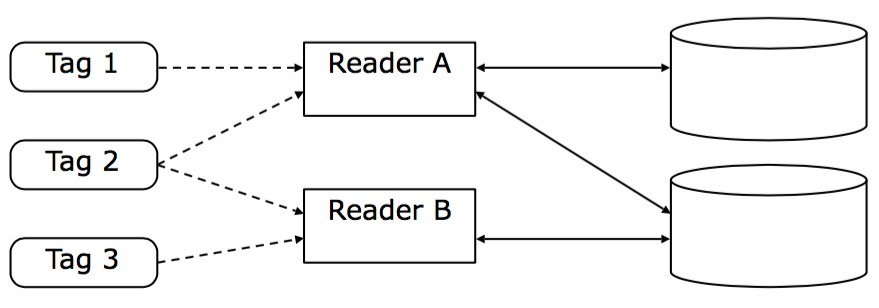
\includegraphics[width=\textwidth]{shema}
\caption{Illustration du système RFID}
\end{figure}
\subsection{Les composants essential d'un system RFID}
\subsubsection{Les tags}
Les tags sont attachés à tous les objets à identifier dans un système RFID. Un tag est généralement
composé d'une antenne ou un élément de couplage, et un circuit intégré. Un important
distinction qui sera discuté plus tard est la source d'alimentation d'un tag. Souvent, les étiquettes ne portent pas une source d'alimentation et doit passivement récolter toute l'énergie d'un signal RF.\\

Il existe plusieurs types de tag qui offrent des fonctionnalités différentes, ont des puissances différentes
de sources ou fonctionnent à des fréquences radio différentes. Chacune de ces variables permet de déterminer
quelles applications une étiquette particulière peut être approprié. Ces différences seront examinées plus loin dans ce chapitre.\\

Les étiquettes modernes ont tendance à mettre en œuvre la fonctionnalité d'identification sur un circuit intégré (IC) qui
assure le calcul et le stockage. Dans le procédé de fabrication, ce circuit intégré est fixé ou
"Attaché" à une antenne avant d'être emballés dans un facteur de forme, comme une capsule de verre ou d'une feuille, qui est intégré dans un produit final.\\
Dans la pratique, les différents fournisseurs effectuent souvent chacune de ces étapes de fabrication. Autres RFID
dessins peuvent être «chipless» ou avoir des informations d'identification au moment de la fabrication, à savoir
"Écriture une fois, lecture nombreuse". \\
\begin{figure}[h!]
\centering
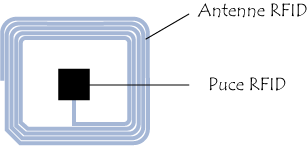
\includegraphics[height=3cm]{tag}
\caption{Tag RFID}
\end{figure}
\subsubsection{Reader/Lecteur}
Les lecteurs RFID communiquent avec des tag à travers un canal RF pour obtenir l'identification
. Selon le type d'étiquette, cette communication peut être un simple ping ou peut être un protocole plus complexe de caractaire multi-tour. Dans les environnements avec de nombreux points, un lecteur peut avoir à effectuer une algorithme d'anti-collision pour veiller à ce que les conflits ne peuvent pas se produire. Les protocoles anti-collision permettent aux lecteurs de communiquer rapidement avec beaucoup de tag en série.

Les lecteurs alimentent souvent ce que l'on appelle les étiquettes passives à travers leur canal de communication RF.
Ces types d'étiquettes ne portent aucune puissance à bord et comptent uniquement sur un lecteur pour fonctionner. Étant donné que ces tag sont si limitées, il compter sur un lecteur pour effectuer des calculs.
Les lecteurs se présentent sous plusieurs formes, fonctionnent sur de nombreuses fréquences différentes, et peuvent offrir un large éventail de fonctionnalités. Les lecteurs peuvent avoir leur propre puissance de traitement et de stockage interne, et peuvent offrir une connectivité réseau. Les lecteurs pourraient être une simple conduit à un système externe, ou pourraient stocker toutes les données pertinentes au niveau local.

À l'heure actuelle, de nombreuses applications reposent sur des dispositifs de lecture fixes. Les premiers essais de EPC à une grande chaîne de supermarchés intégrés dans les lecteurs entrées accueil baies fixes. Ces lecteurs scannent les étiquettes au niveau de la palette que les livraisons de produits arrivent. 

À long terme, les lecteurs peuvent être intégrés à un niveau d'étagère comme une «étagère intelligente». étagères intelligentes seraient scanner pour les balises au niveau de l'article et de surveiller quand ils sont ajoutés et supprimés d'une étagère.

Les lecteurs RFID peuvent également être intégrés dans des appareils mobiles portatifs. Ces lecteurs mobiles permettraient à quelqu'un, par exemple, faire l'inventaire d'un entrepôt en marchant à travers ses allées. Le fabricant de téléphone cellulaire Nokia propose déjà des fonctionnalités RFID de lecture dans certains de leurs téléphones cellulaires [16]. Si les balises de type EPC deviennent très réussie, intéressante et les applications grand public utiles pourraient se poser. Si cela se produit, la fonctionnalité de lecture RFID pourrait devenir une caractéristique commune sur les téléphones, PDA, ou d'autres dispositifs informatiques portables cellulaires
\begin{figure}[h!]
\centering
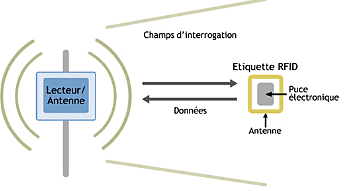
\includegraphics[height=4cm]{reader}
\caption{Interaction du Lecteur RFID avec son environement}
\end{figure}
\subsubsection{La bases de donnée}
bases de données RFID associent l'identifiant de tag avec un enregistrements. Ces enregistrements peuvent contenir des informations sur les produits, les journaux de suivi, les données de ventes, ou les dates d'expiration. Des bases de données indépendantes peuvent être construites tout au long de la chaîne d'approvisionnement par des utilisateurs indépendants, ou peuvent être intégrés dans un système de base de données centralisée ou fédérée.\\

Les bases de données sont supposées avoir une connexion sécurisée aux lecteurs. Bien qu'il existe des scénarios où les lecteurs peuvent ne pas être dignes de confiance, il est souvent utile de faire écrouler les notions de lecteur et la base de données en une seule entité. Par exemple, si les étiquettes contiennent toutes les informations de produits en cause, il n'y a pas besoin de faire un appel à une base de données hors site.
On peut imaginer un système fédéré de bases de données back-end, peut-être où chaque fabricant de produit conserve son propre service de consultation produit. Dans ces paramètres, il peut être utile de déployer un service Object Naming (ONS) pour localiser les bases de données associées à une valeur d'identification d'étiquette. Un ONS permet au lecteur de trouver un ensemble de bases de données associées à une valeur d'identification d'étiquette particulière. Ceci est analogue à l'Internet Domain Naming Service (DNS) qui renvoie les adresses des serveurs de noms qui peuvent se traduire les noms de domaine en adresses IP numériques. ONS n'a pas encore été largement adopté dans la pratique.
\subsection{Source d'énergie d'un Tag}
Comme brièvement mentionné précédemment, les étiquettes peuvent obtenir leur pouvoir de plusieurs manières différentes. La source d'énergie est une propriété essentielle d'une étiquette, car il va déterminer la distance de lecture potentielle d'une balise, la durée de vie, le coût, et quel genre de fonctionnalités qu'il peut offrir. La source d'énergie sera également important pour déterminer comment une étiquette peut être orienté et quelles formes physiques qu'il peut prendre.Il existe trois catégories principales de sources d'énergie de tag: actifs, semi-passifs, et passifs.\\

 Les étiquettes actives ont leur propre source d'énergie, telle qu'une batterie, et peuvent initier une communication à un lecteur ou d'autres balises actives. Parce qu'ils contiennent leur propre source d'alimentation, les étiquettes actives ont généralement une plage de fonctionnement beaucoup plus large que passifs-tags. Une caractéristique clé de balises actives est qu'ils sont en mesure de lancer leur propre communication avec les lecteurs. Les balises actives avancées, pourraient même former des réseaux ad hoc les uns avec les autres. Une application utile est les balises actives dans des conteneurs d'expédition , qui peuvent tomber hors navires sur les mers agitées. Ces conteneurs manquants parfois ne sont pas reconnus jusqu'à ce que le navire à quai . Une étiquette à puce avec un capteur accéléromètre pouvait détecter quand il est tombé et distribuer un journal de sa disparition avant de sombrer dans l'océan.\\
 
Par contre, un semi-passif (ou semi-actif) tag ont une batterie interne, mais ne sont pas en mesure d'initier des communications. Cela garantit que les étiquettes semi-passives ne sont actives que lorsqu'il est interrogé par un lecteur. Parce que les étiquettes semi-passives ont une source d'énergie interne, ils offrent une lecteur plus large que les passives, mais à un coût plus élevé.
Un exemple d'application qui utilise souvent des étiquettes semi-passives est \emph {tollbooths} électroniques. les étiquettes passives sont généralement collée à l'intérieur du pare-brise d'une voiture. Lorsque la voiture passe par un péage, il lancera une requête à l'étiquette et lire un compte identifiant de l'étiquette. La batterie de bord permet la balise être lues à une distance considérable. Cependant, étant donné que l'étiquette ne doit diffuser lorsqu'il est interrogé, il peut rester inactif la plupart du temps et économiser de l'énergie. Les étiquettes semi-passives sont également souvent utilisés dans les palettes au niveau de suivi ou de suivi des composants tels que des pièces d'automobile lors de la fabrication.\\

Les étiquettes passives ont ni leur propre source d'énergie, ni la capacité d'initier la communication. Les étiquettes passives obtiennent de l'énergie par la récolte à partir d'un signal de communication RF entrant. À des fréquences plus basses, cette énergie est typiquement récoltées par induction, tandis qu'à des fréquences plus élevées, il est récolté par capacité.

Bien que les étiquettes passives ont la plus courte distance de lecture de tous les trois types alimentant, ils sont les moins chers à fabriquer et plus facile à intégrer dans des produits. Les batteries sont relativement coûteux et ne peuvent pas facilement être incorporés dans certains articles, comme les emballages en papier. Pour cette raison, les étiquettes passives sont des balises les plus courantes.

En l'absence d'une source d'énergie interne dicte de nombreuses propriétés des étiquettes passives. D'abord, ils ne peuvent pas fonctionner sans la présence d'un lecteur, bien que étiquette passive pourrait temporairement en cache un peu d'énergie dans un condensateur. En raison de leur faible nécessairement signal de réponse, les étiquettes passives sont souvent plus sensibles au bruit ambiant ou des interférences. Le tableau 1 compare diverses propriétés des étiquettes passives, semi-passives et actives.\\

\begin{longtable}{|p{0.35\textwidth}|p{0.2\textwidth}|p{0.2\textwidth}| p{0.15\textwidth}| p{0.15\textwidth}|}
\hline
\textbf{Type} & \textbf{Passif} & \textbf{Semi-Passif} & \textbf{Active} \\
\hline
\textbf{Source d'énergie} & énergie récolté du RF & Batterie & Batterie \\
\hline
\textbf{Communication} & Réponse seulement & Réponse seulement & Répondre ou initier \\
\hline
\textbf{Max Range} & 10 M & 100 M &  100 M \\
\hline
\textbf{Coût relatif} & Le moins cher & Plus cher & Très cher \\
\hline
\textbf{Exemple Applications} & EPC cartes de proximité & télé péage &  \emph {Livestock tracking} \\
\hline
\caption{Comparaison de tag passif , semi- passif et actif}
\end{longtable}


\subsection{Fréquences de fonctionnement}
Les systèmes RFID a une variété de fréquences radio. Chaque bande de fréquences offre sa propre avantage d'exploitation, les exigences de puissance et de performance. Différentes gammes peuvent être soumis à des règlements ou des restrictions qui limitent ce que les applications peuvent être utilisés pour.
Les métaux et les liquides présentent généralement le plus gros problème dans la pratique. En particulier, les balises actives dans l'ultra-haute fréquence (UHF) ne fonctionnent pas correctement à proximité de liquides ou de métal.

Fréquence de fonctionnement est également important dans la détermination des dimensions physiques d'une étiquette RFID. Différentes tailles et formes des antennes fonctionnent à des fréquences différentes. La fréquence de fonctionnement détermine également la possibilité d'interagir physiquement avec les autres. Par exemple, l'empilage des étiquettes plates feuille d'incrustation sur le dessus de l'autre peut interférer ou empêcher les balises de la lecture correctement. Le tableau 2 énumère les fréquences standard et leurs distances de lecture passifs respectifs.\\
\begin{longtable}{|p{0.35\textwidth}|p{0.2\textwidth}|p{0.2\textwidth}|}
\hline
\textbf{Gamme de fréquences} & \textbf{fréquences} & \textbf{Distance de lecture} \\
\hline
Basse fréquence & 120-140 KHz & 10-20 cm  \\
\hline
Haute Fréquence (HF) & 13,56 MHz & 10-20 cm \\
\hline
Ultra-haute fréquence (UHF) & 868-928 MHz & 3 mètres \\
\hline
Micro onde & 2,45 et 5,8 GHz & 3 mètres \\
\hline
Ultra-Wideband (UWB) & 3,1-10,6 GHz & 10 m \\
\hline
\caption{fréquences de fonctionnement RFID}
\end{longtable}
\subsubsection{Basse fréquence (LF)}
Basse fréquence (LF) étiquettes RFID fonctionnent généralement dans la gamme 120-140 kilohertz. Le plus souvent, les balises LF sont passivement alimentés par induction. En conséquence, ils ont généralement de très courts intervalles de lecture 10-20 centimètres.

Les balises LF peuvent être utilisés dans des environnements difficiles et peuvent fonctionner à proximité de métal, des liquides, ou de la saleté. Cela les rend utiles pour des applications comme les étiquettes d'identification pour animaux de compagnie implantables ou des étiquettes de gestion de blanchisserie. Un inconvénient de balises LF est qu'ils ont une très faible taux de lecture de données par rapport à d'autres fréquences de fonctionnement.

LF balises sont souvent utilisés dans les systèmes d'immobilisation de la voiture et de contrôle d'accès. Dans ces systèmes, une voiture ne démarre que si une balise de LF, généralement attaché à la clé de contact, est à proximité de l'allumage. Cela prend avantage de courte portée de lecture de LF et l'utilise comme un élément de sécurité.

En 20016, LF étiquettes passives peuvent être achetés en vrac pour 10 DH par tag ou moins. Deux grands fabricants de balises LF sont Texas Instruments et Phillips Semiconductor. La norme \emph{ISO 18000-2 standard} [11] offre des spécifications pour les étiquettes RFID LF.

\subsubsection{Haute fréquence}
Haute fréquence (HF) étiquettes RFID fonctionnent à la fréquence de 13,56 MHz. étiquettes HF sont souvent emballés dans un facteur d'incrustation de feuille ou sous forme de carte de crédit. Cela rend les balises HF utiles pour la construction de contrôle d'accès, les cartes de crédit sans contact, et des badges d'identification. Encore une fois.

Les étiquettes HF sont également utilisés dans de nombreuses applications de suivi. Les bibliothèques et les librairies utilisent souvent HF incrustations de feuilles pour suivre les livres. Certains aéroports ont commencé à utiliser HF RFID étiquettes à bagages pour les applications de manutention de bagages.

les étiquettes HF offrent un taux de lecture de données plus élevé que les balises LF, mais ne réussissent pas aussi bien que les balises de LF à proximité de métaux ou de liquides. balises HF font, cependant, offrent de meilleures performances à proximité de métaux ou de liquides que les tags UHF font.

La gamme de fréquence HF se trouve sur une partie fortement réglementée du spectre radio. Les signaux transmis par les lecteurs doivent fonctionner dans une bande de fréquence étroite. Cela pose un problème pour les environnements électroniques sensibles, tels que les équipements médicaux, qui fonctionnent sur des fréquences voisines. Cela rend les balises HF inappropriée pour les environnements comme les hôpitaux.

En 2016, HF étiquettes passives peuvent être achetés pour 5DH ou moins par étiquette en quantité. Texas Instruments et Phillips offrent tous deux lignes tag HF, bien qu'il existe de nombreux fabricants plus petits et spécialisés ou intégrateurs dans l'espace de HF.
Organisation internationale de normalisation (ISO) spécifications pour les étiquettes RFID HF sont spécifiées par la norme \emph{ISO 18000-3 norme} [11]. spécifications connexes HF sans contact des cartes à puce et les cartes de proximité apparaissent dans les normes ISO 14443 [9] et 15693 [10].
\subsubsection{Ultra-haute fréquence}
Ultra-haute fréquence (UHF) étiquettes RFID fonctionnent dans la gamme de 868 à 928 mégahertz. balises européennes fonctionnent généralement dans la gamme 868-870 MHz, tandis que les États-Unis et au Canada fonctionnent à 902-928 MHz. tags UHF sont les plus couramment utilisés pour les applications de suivi et de gestion de la chaîne logistique article. Ceci est en grande partie parce qu'ils offrent une gamme plus lu et sont moins chers à fabriquer en vrac que LF ou HF tags. Les étiquettes EPC de première génération fonctionnent à des fréquences UHF.

Un inconvénient majeur de tags UHF est qu'ils éprouvent des interférences à proximité de liquides ou de métaux. De nombreuses applications telles que le suivi des animaux, suivi des conteneurs en métal, ou même de nombreux systèmes de contrôle d'accès sont irréalisables avec des étiquettes UHF. Certains matériaux ont été développés qui peuvent protéger les tags UHF de distorsion liés à métal, mais ceux-ci peuvent être coûts prohibitifs à utiliser dans la pratique. lecteurs UHF peuvent également interférer avec l'électronique sensible comme l'équipement médical.

tags UHF sont une technologie relativement récente que LF ou HF, et les coûts de lecteur sont généralement plus élevés que les lecteurs de LF faible largeur de bande. En 2016, les tags UHF peuvent être achetés en quantités pour moins de 1DH par étiquette passive. étiquettes UHF coûts aussi bas  0.5DH sont susceptibles d'arriver sur le marché dans les prochaines années. Spécifications pour les étiquettes RFID fonctionnant à des fréquences UHF sont définies à la fois par l'ISO 18000-6 [11] et à la norme EPCGlobal [6].
\subsubsection{Micro-ondes} 
étiquettes de micro-ondes fonctionnent soit à 2,45 ou 5,8 gigahertz. Cette gamme de fréquences est parfois appelée fréquences de super-haute (SHF). La technologie RFID de micro-ondes est entré en usage assez récemment et se développe rapidement. étiquettes à micro-ondes utilisées dans la pratique sont généralement semi-passif ou actif, mais peuvent aussi se présenter sous forme passive. balises à micro-ondes semi-passives sont souvent utilisés dans l'identification de la flotte et des applications de télépéage.
Les systèmes à micro-ondes offrent plus les taux de lecture que UHF et gammes équivalentes de lecture passive. Plages de lecture semi-passives et actives des systèmes de micro-ondes sont souvent plus grandes que leurs homologues UHF. Certains micro-ondes balises actives peuvent être lues à partir des distances allant jusqu'à 30 mètres, ce qui est moins de tags UHF comparables. Cependant, les implémentations physiques des micro-ondes étiquettes RFID peuvent être beaucoup plus petit et compact que basse fréquence des étiquettes RFID.
Il y a plusieurs inconvénients à des balises à micro-ondes. La première est qu'ils consomment relativement plus d'énergie que leurs homologues de fréquence inférieure. étiquettes de micro-ondes sont généralement plus chers que les tags UHF. Commercialement balises actives disponibles coûtent autant que 250 DH par tag en 2016.
Un autre problème est que le sans fil 802.11b / g réseaux (WiFi) peuvent interférer avec les systèmes micro-ondes RFID. Dispositifs d'application de la ZigBee 802.15 prochaine norme sans fil pourraient potentiellement entrer en conflit avec des dispositifs micro-ondes RFID ainsi.
L'ISO 18000-4 et ISO 18000-5 rejeté [11] Les normes offrent des spécifications respectives pour 2,45 et 5,8 gigahertz étiquettes RFID.
\subsubsection{Ultra-Wideband}
Ultra-wideband (UWB) appliquée à la RFID est assez récente. Plutôt que d'envoyer un signal fort sur une fréquence particulière, UWB utilise des signaux de faible puissance sur une très large gamme de fréquences. Le signal sur une fréquence particulière utilisée par UWB est très faible, mais dans l'ensemble, la communication est assez robuste. Dans la pratique, certaines implémentations de UWB fonctionnent de 3,1 à 10,6 GHz.
Les avantages de l'UWB sont qu'il a une très longue portée en ligne de mire de lecture, peut-être 200 mètres dans certains contextes. UWB est également compatible avec le métal ou les liquides. Comme le signal sur une fréquence particulière est très faible, UWB ne pas interférer avec les équipements sensibles. Par conséquent, une application anticipée était suivi des actifs dans un milieu hospitalier.
Un inconvénient d'implémentations actuelles de UWB est qu'il doit être actif ou au moins semi-passive. Cependant, étant donné que les balises UWB diffusent des signaux très faibles, ils ont relativement faible consommation d'énergie. En 2006, il est difficile de savoir si la technologie existe pour créer un UWB tag2 passive.
La technologie RFID UWB est encore dans ses premières phases et il y a peu de produits disponibles dans le commerce. Les coûts de 50DH par tag en vrac sont raisonnables dans un proche avenir.
\subsection{Fonctionnalité}
La fonctionnalité RFID de base est l'identification. Lorsqu'il a été interrogé par un lecteur, les balises retournent un autre identificateur qui peut être utilisé pour récupérer d'autres enregistrements de données. Cependant, les étiquettes peuvent offrir d'autres fonctionnalités utiles dans différentes applications. Les principes et les technologies de ces différents types de balises sous-jacentes sont si étroitement liés aux étiquettes RFID strictes, qu'ils ont souvent collectivement appelés «RFID». Bien que pas strictement RFID, nous discutons de plusieurs classes majeures d'appareils liés à la RFID.

Nous avons partagé des étiquettes RFID de style en cinq grandes catégories: EAS, en lecture seule EPC, EPC, étiquettes de capteurs, et motes. Ceux-ci seront appelés classes A à E. EPCglobal propose cinq classes similaires de tag basé sur la fonctionnalité baptisée classe 0 à la classe 4 [6]. Les classes EPCglobal aligner étroitement avec les nôtres, mais diffèrent quelque peu. Ces cinq classes sont résumés dans le tableau 3.\\

\begin{longtable}{|p{0.1\textwidth}|p{0.2\textwidth}|p{0.2\textwidth}| p{0.15\textwidth}|p{0.2\textwidth}|}
\hline
\textbf{Classe} & \textbf{Nom} & \textbf{Mémoire} & \textbf{Source d'énergie} & \textbf{Caractéristi-ques} \\
\hline
A & EAS & Aucun & Passif & article surveillance \\
\hline
B & Lecture seule EPC & Lecture seulement & Passif & identification seulement \\
\hline
C & EPC & Lire et écrire & Passif & Enregistrement de données \\
\hline
D & capteur Balises & Lire écrire & Semi-passif & capteurs environnementaux \\
\hline
E & motes & Lire écrire & actif & Réseautage ad hoc \\
\hline
\caption{Classes de fonctionnalité des Tags}
\end{longtable}

\subsection{Normes}

Les deux normes RFID les plus pertinents sont l'Organisation internationale de la norme ISO / IEC 18000 de normalisation norme [11] et les normes de EPCglobal [6]. Ces normes ne sont pas en concurrence, et il est concevable que la norme EPCglobal pourrait éventuellement être adopté dans une norme ISO.
EPCglobal définit des spécifications pour les étiquettes de type EPC fonctionnant dans la gamme UHF.
La norme ISO 18000 a 6 parties d'adressage différentes gammes de fréquences:
\begin{itemize}
\item Partie 1 - Généralités normes
\item Partie 2 - LF
\item Partie 3 - HF
\item Partie 4 - Micro-ondes, 2,45 GHz
\item Partie 5 - Micro-ondes, 5,8 GHz
\item Partie 6 - UHF\\
\end{itemize}
\subsection{Modes de transfert d’énergie et de communication}
Dans ce premier cas ( figure 3.4) , l’onde RF se propageant de la base station vers le tag n’a pour but unique que de fournir de l’énergie au tag de façon à charger la  capacité d’alimentation  présente à son bord afin que celle-ci puisse être capable d’alimenter l’ensemble du tag pour assurer son bon fonctionnement. Aprés cette phase d'alimentation, le tag est apte à recevoir des ordres de commande provenant de la base station et de retourner des informations vers celle-ci. Puis le cycle recommence et il est à nouveau nécessaire de lui fournir de l'énergie pour continuer la communication et ainsi de suite. Bien évidemment, ceci prend du temps et manque parfois de souplesse.\\
\begin{figure}[h!]
\centering
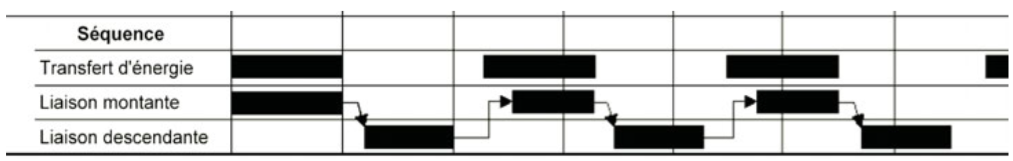
\includegraphics[width=\textwidth]{figa}
\caption{Mode de transfert d'énergie non simultané}
\end{figure}

Dans ce deuxième cas ( figure 3.5), au travers des principes et types de modulation utilisés, l'onde provenant de la base station est capable pendant la phase de l'échange base station vers tag d'assurer simultanément la fourniture de l'énergie et l'échange des informations (données).\\

\begin{figure}[h!]
\centering
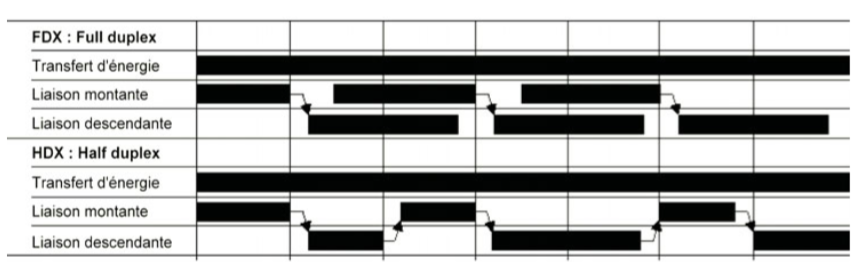
\includegraphics[width=\textwidth]{figb}
\caption{Mode de transfert d'énergie simultané}
\end{figure}

\begin{center}
\textbf{\emph{Note :}}\\
\emph{À noter que la trés grande majorité des tags du commerce fonctionnent selon ce dernier principe.}
\end{center}

\subsection{Liaison montante et liaison descendante}
Intéressons-nous d’abord aux échanges ayant lieu entre bases stations et tags. Ils sont de deux sortes et seront définis une fois pour toutes dans cet ouvrage de la manière suivante :
\begin{itemize}
\item de la base station vers le tag, dits liaison montante ;
\item du tag vers la base station, dits liaison descendante. \\
\end{itemize}
De plus afin d’éviter quelques problèmes de compréhension, quelle que soit l’intelligence embarquée dans le tag, nous supposerons que celui-ci ne fonctionne que sous des ordres commandes provenant de la base station. 
\subsubsection{Liaison montante ( forward link) de la base station vers le tag}
La liaison montante (de la base station vers le tag) a pour mission :
\begin{itemize}
\item d'assurer, si cela est possible, le transport de l'énergie vers le tag afin que celui-ci puisse assurer la taÌ‚che qui lui incombe ;
\item de servir de support à l'envoi de données de la base station vers le tag ;
\item d'assurer, si cela est possible, le transport de l'énergie vers le tag afin que celui-ci puisse assurer
\item dans le cas des systèmes fonctionnant en mode passif (voir définition un peu plus loin), lors de la phase de communication en liaison descendante, d'assurer la présence d'un support physique à la communication du tag vers la base station.
\end{itemize}
La communication montante est par principe assurée par un dispositif – la base station – qui émet une onde radiofréquence. Celle-ci est donc dotée d’un émetteur, un TRANSmitter. De par la présence de cet émetteur, la liaison montante est dite active. De plus, la base station comporte également à son bord un récepteur, un reCEIVER. La base station est donc un TRANSCEIVER. Dans le sens montant, la base station doit se faire comprendre par le tag au travers d’un co- dage numérique (binaire), d’un protocole de communication et d’un système de modulation de la fréquence porteuse ne devant pas ou peu affecter (le plus faiblement possible) la qualité d’une hypothétique télé-alimentation simultanée. Pour cela on peut employer des techniques de modulation de fréquence FSK \footnote{Frequency-Shift Keying}, ou encore de nombreuses méthodes de modulation d’amplitude ASK \footnote{Amplitude-Shift Keying}
\subsubsection{Liaison descendante de la modulation}
Contrairement à ce qu'on pourrait initialement penser, le transpondeur ne peut pas se comporter comme un émetteur de signaux RF. En effet, il ne dispose pas, dans son interface RF, des mécanismes permettant d'émettre un signal radio-fréquence vers la station de base.Les transpondeurs utilisent ce qu'on appelle la réflexion d'ondes pour se faire comprendre des lecteurs. \\

Pour cela, les tags utilisent une modulation différente que l'on nomme modulation de charge (Load Modulation) qui consiste à faire varier la charge résistive du circuit. Effectivement, en faisant varier la charge, le tag fait varier l'intensité du courant dans son circuit et donc l'intensité qui circule dans l'antenne. La consommation d'énergie qu'il représente dans le champ magnétique s'en trouve alors également modifiée et, par couplage magnétique, cela influe sur l'intensité du courant dans l'antenne de la station de base. De proche en proche, les signaux RF reçus de la station de base, qui sont réfléchis par le transpondeur, permettent donc de transporter des réponses en faisant varier l'intensité du circuit du lecteur.\\

Il s'agit ici d'un procédé assez complexe mais qui repose à la base sur de la modulation. Cette modulation de charge résistive à l'origine de la transmission de la réponse s'appuie sur une modulation courante appelée OOK \footnote{On Off Keying} et correspond à la modulation d'amplitude "tout ou rien". A l'aide d'une modulation de type OOK, comme présentée précédemment, on crée une modulation de charge qui fait varier la charge résistive du circuit et donc la tension aux bornes du circuit RF du transpondeur comme montré dans la figure 3.5.

\begin{figure}[h!]
\centering
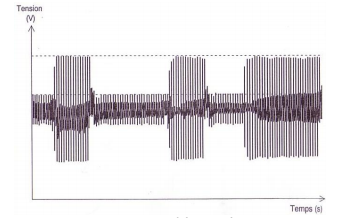
\includegraphics[width=\textwidth]{ook}
\caption{On Off Keying}
\end{figure}
\end{document}